\begin{itemize}
\item[$\blacktriangleright$] Open up Eclipse with a clean, fresh workspace. Go to ``Window/Open Perspective/Other\ldots'' \footnote{A path given as ``foo/bar'' indicates how to navigate in a series of menus and submenus.} and choose eMoflon~(Fig.~\ref{fig_eclipse}).

\begin{figure}[htbp]
	\centering
  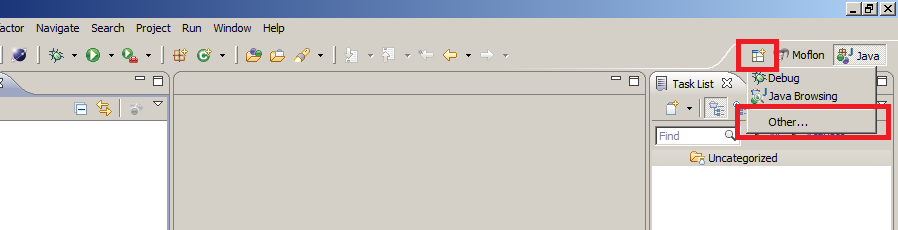
\includegraphics[width=\textwidth]{eclipse_firststart}
	\caption{Choose the Moflon perspective.}
	\label{fig_eclipse}
\end{figure} 

\item[$\blacktriangleright$] In the far right toolbar, a new action set should have appeared. Choose ``New Metamodel'' (Fig.~\ref{fig_eclipseNewMetamodel}).
\footnote{The button with an `L' shows you our logfile (important input for us if something goes wrong!). You remember our email address, right?}

\begin{figure}[htbp]
	\centering
  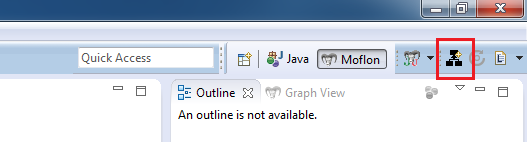
\includegraphics[width=\textwidth]{eclipse_newMetamodelOne}
	\caption{Eclipse ''New Metamodel''}
	\label{fig_eclipseNewMetamodel}
\end{figure}
 
\item[$\blacktriangleright$] Name the project `Demo' and select `Visual (Enterprise Architect)' . Make sure that 'Add Demo Specification' is checked off! 

\end{itemize}